\documentclass[tikz,border=4pt]{standalone}
\usepackage{amsmath}
\begin{document}
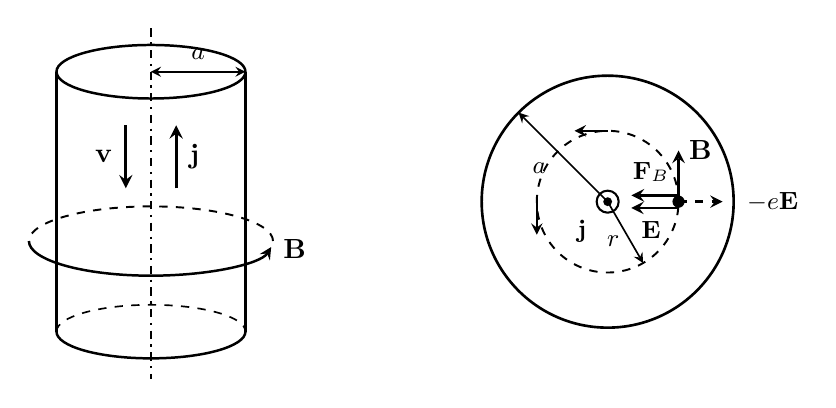
\begin{tikzpicture}[>=stealth, thick, scale=1.0]
  % Left panel: Perspective side view of cylindrical wire
  \begin{scope}[xshift=0cm]
    % Cylinder walls
    \draw[line width=0.9pt] (-1.2, 1.8) -- (-1.2, -1.5);
    \draw[line width=0.9pt] (1.2, 1.8) -- (1.2, -1.5);
    \draw[line width=0.9pt] (0, 1.8) ellipse (1.2 and 0.34);
    \draw[line width=0.9pt] (-1.2, -1.5) arc (180:360:1.2 and 0.34);
    \draw[dashed, line width=0.6pt] (-1.2, -1.5) arc (180:0:1.2 and 0.34);

    % Center axis
    \draw[dash dot, line width=0.55pt] (0, 2.35) -- (0, -2.1);

    % Current density j (upward) and electron drift velocity v (downward)
    \draw[->, line width=1.1pt] (0.32, 0.32) -- (0.32, 1.12);
    \node[right] at (0.36, 0.72) {$\mathbf{j}$};
    \draw[->, line width=1.1pt] (-0.32, 1.12) -- (-0.32, 0.32);
    \node[left] at (-0.36, 0.72) {$\mathbf{v}$};

    % Azimuthal magnetic field B loop around the cylinder (counterclockwise from above)
    \draw[->, line width=0.9pt] (-1.55, -0.35) arc (180:350:1.55 and 0.44);
    \draw[dashed, line width=0.7pt] (1.55, -0.35) arc (0:180:1.55 and 0.44);
    \node[right] at (1.55, -0.45) {$\mathbf{B}$};

    % Radius a marker
    \draw[<->, line width=0.6pt] (0, 1.8) -- (1.2, 1.8);
    \node[above, font=\small] at (0.6, 1.82) {$a$};
  \end{scope}

  % Right panel: Top cross-section (current j coming out of page, electron v going into page)
  \begin{scope}[xshift=5.8cm, yshift=0.15cm]
    % Wire cross section (radius 1.60)
    \draw[line width=0.95pt] (0, 0) circle (1.60);
    % Inner circle of radius r = 0.90
    \draw[dashed, line width=0.7pt] (0, 0) circle (0.90);

    % Center symbol for j (out of page: circle with dot)
    \draw[line width=0.75pt] (0, 0) circle (0.14);
    \fill (0, 0) circle (1.6pt);
    \node[below left, font=\small] at (-0.14, -0.10) {$\mathbf{j}$};

    % Azimuthal B arrows (counterclockwise) on inner circle
    \draw[->, line width=1.0pt] (0.90, 0) -- (0.90, 0.65) node[right] {$\mathbf{B}$};
    \draw[->, line width=0.8pt] (0, 0.90) -- (-0.42, 0.90);
    \draw[->, line width=0.8pt] (-0.90, 0) -- (-0.90, -0.42);

    % Electron point at (0.90, 0)
    \fill (0.90, 0) circle (2.2pt);

    % Radial inward Lorentz force F_B and balancing E (both inward)
    \draw[->, line width=1.05pt] (0.90, 0.08) -- (0.30, 0.08);
    \node[above, font=\small] at (0.55, 0.12) {$\mathbf{F}_B$};
    \draw[->, line width=0.95pt] (0.90, -0.08) -- (0.30, -0.08);
    \node[below, font=\small] at (0.55, -0.12) {$\mathbf{E}$};

    % Electric force -eE outward
    \draw[->, line width=0.95pt, dashed] (0.90, 0) -- (1.46, 0);
    \node[right, font=\small] at (1.64, 0) {$-e\mathbf{E}$};

    % Radius labels a and r
    \draw[->, line width=0.6pt] (0, 0) -- (-1.131, 1.131);
    \node[below left, font=\small] at (-0.65, 0.62) {$a$};
    \draw[->, line width=0.6pt] (0, 0) -- (0.45, -0.779);
    \node[left, font=\small] at (0.28, -0.50) {$r$};
  \end{scope}
\end{tikzpicture}
\end{document}
